\documentclass[11pt,a4paper]{article}
\usepackage[utf8]{inputenc}
\usepackage{hyperref}
\usepackage{minted}
\usepackage{tikz}
\usepackage{graphicx}

\usetikzlibrary{decorations.pathreplacing}

\usepackage{todonotes}

\setmintedinline{breaklines}
\setminted{breaklines}

\newcommand{\warning}[1]{
\noindent
\fbox{
\begin{minipage}{0.1\linewidth}
\raisebox{-6em}{
\scalebox{3}{%
\makebox[2.1em][c]{%
\makebox[0pt][c]{\raisebox{0.3em}{\large!}}%
\makebox[0pt][c]{\color{red}\Huge$\bigtriangleup$}}}
}
\end{minipage}
\begin{minipage}{0.1\linewidth}
\hfill
\end{minipage}
\begin{minipage}{0.7\linewidth}
\vspace{1em}
#1
\vspace{1em}
\end{minipage}
\begin{minipage}{0.05\linewidth}
\hfill
\end{minipage}
}
}

\title{Introducing Bluetooth Low Energy}
\author{Kolbjørn Austreng}
\date{}

\begin{document}
\maketitle

\renewcommand{\thesection}{\roman{section}}
\renewcommand{\thesubsection}{\roman{section}.\alph{subsection}}

\section{Introduction}
Wired protocols are all well and nice - and although CAN is a relatively old protocol now partly superseded by CAN FD (ISO 11898); it is still widely used today. Nevertheless, wireless protocols are becoming increasingly popular wherever they can be used, due to their low cost, and ease of use.\\
\\
One such protocol - Bluetooth 4.2, or Bluetooth Low Energy (BLE for short), is almost certainly supported by your smart phone; as well as a plethora of different devices that we interact with daily. This makes it an ideal candidate for introducing wireless connectivity to your project - of course provided you can live with the interference present in the 2.4 GHz ISM band.\\
\\
Many of the students taking this course will previously have had the course "Embedded Systems" (TTK4235), in which the \textit{micro:bit} development board was used during the labs. This is an excellent platform for introducing the Bluetooth Low Energy stack, and we will be using the micro:bit platform in this course as well. TTK4235 is no prerequisite, and it should be straight forward to follow this lab assignment without having gone through that course.\\
\\
If no one on your group has a micro:bit, you may talk to one of the student assistants. It is also possible to use other hardware, such as an nRF52DK if you happen to have one, but bear in mind that other hardware platforms support different Application Programming Interfaces (APIs) for the Bluetooth stack.\\
\\
This assignment was developed on Linux. It should be relatively straight forward to follow along with other platforms using the GNU toolchain as well, but keep in mind that you will be slightly more on your own in that case.

\newpage
\noindent
\section{Initial Setup of Hardward and Toolchain}
The following hardware configuration is only necessary for those of you who have not already done so through TTK4235. However, it might still be necessary to set up the toolchain, as nothing is certain when it comes to the computers at the real time lab.

\subsection{Hardware Configuration}
By default, the micro:bit comes preloaded with a custom Device Abstraction Layer (DAL) that allows programming the device through Scratch, Micropython, or JavaScript. This is well for simple demonstrations, but yields no control of the low level hardware. To get around this limitation, we will upgrade the flasher circuit to use the BBC micro:bit J-Link OB Firmware.

\begin{enumerate}
\item Download the \href{https://www.segger.com/downloads/jlink#BBC\_microbit}{J-Link OB Firmware from Segger.com}\footnote{https://www.segger.com/downloads/jlink\#BBC\_microbit}.
\item Start with the micro:bit unplugged. While holding down the Reset button (next to the USB connector), connect it to the computer.
\item The micro:bit should now have mounted itself as "MAINTENANCE" on the file system. You can now let go of the Reset button.
\item Move the .hex-file that you downloaded into "MAINTENANCE".
\item The micro:bit should now automatically remount after a few seconds; this time as "MICROBIT".
\end{enumerate}

\subsection{Toolchain Configuration}
\label{sec::toolchain_config}
To compile and flash code for the micro:bit, we need to install a toolchain. For compilation, GCC is a natural choice. Since the heart of the micro:bit is an nRF51822, we will be using J-Link and nrfjprog to flash the board.

\begin{enumerate}
\item Call \mintinline{text}{nrfjprog --version} to see if the toolchain is already set up on the computer. If it is, you may skip the remaining steps.
\item Call \mintinline{text}{sudo apt install gcc-arm-none-eabi} to install the GCC ARM compiler.
\item Go to \href{https://www.nordicsemi.com/eng/nordic/Products/nRF51822/nRF5x-Command-Line-Tools-Linux64/51386}{nordicsemi.com}\footnote{https://www.nordicsemi.com/eng/nordic/Products/nRF51822/nRF5x-Command-Line-Tools-Linux64/51386} and download the newest version of the nRF command line tools.
\item The download contains the programs \mintinline{text}{nrfjprog} and \mintinline{text}{mergehex}, both must be available in the Linux \mintinline{text}{PATH} variable. This can be done in many ways, here is one:
\begin{enumerate}
\item Extract the \mintinline{text}{nrfjprog}- and \mintinline{text}{mergehex} folders to the home folder.
\item Add the following string at the bottom of the \mintinline{text}{~/.bashrc} file: \mintinline{bash}{"export PATH=$HOME/nrfjprog:$HOME/mergehex:$PATH"} (do not include the quotation marks)%$
\item Finally, since \mintinline{text}{~/.bashrc} is read once when a terminal opens, you need to close and reopen all terminal windows that you might have active.
\end{enumerate}
\item Go to \href{https://www.segger.com/downloads/jlink/\#J-LinkSoftwareAndDocumentationPack}{segger.com}\footnote{https://www.segger.com/downloads/jlink/\#J-LinkSoftwareAndDocumentationPack} and download the J-Link Software and Documentation pack. You should choose the Linux 64 bit version, DEB installer.
\item Once you have downloaded the DEB package, navigate to the download location with a terminal, and call the following command to install the package: \mintinline{text}{sudo dpkg -i JLink_Linux[...]x86_64.deb}
\end{enumerate}

\subsection{Hardware and Toolchain Verification}
First off, you should call \mintinline{text}{nrfjprog --version} to see if the toolchain is set up. If this command complains, you will need to repeat section \ref{sec::toolchain_config}.\\
\\
On Blackboard, you can find an example .hex-file, aptly named "example.hex". To flash this file to the micro:bit, navigate to the directory where you have the hex, and call:
\begin{minted}{bash}
nrfjprog -f nrf51 --chiperase --program example.hex --reset
\end{minted}
The micro:bit should now start broadcasting the name "u:bit" over Bluetooth. To verify this, you may use your phone, as described in section \ref{sec::phone_verify}.

\section{Use your phone for testing}
\label{sec::phone_verify}
You are free to use whatever to check your Bluetooth connection, but an easy choice is to download the "nRF Connect" app for your smart phone. This lab assignment will use that app.\\
\\
When you open nRF Connect, your phone will start scanning for advertising packets, as seen in figure \ref{fig::example_scanning}. You can adjust the RSSI filter (signal strength) to only show devices that are close to you. In the image, this filter is set to $-80$ dBm, but setting it to around $-60$ dBm is probably better if there are a lot of Bluetooth devices nearby.\\
\\
When you connect to the micro:bit, you will see something similar to figure \ref{fig::example_services}. The names "LED Matrix" and "Buttons" will not show up by default, but may be assigned by you, by long-pressing on the \textit{characteristic} and editing the name. Either way, the name of the characteristic is merely cosmetic.\\
\\
By uploading a byte different than 0x00 to the "LED Matrix" characteristic, the LED matrix should turn on; and it should turn off when you upload 0x00.\\
\\
The "Buttons" characteristic contains the state of the two micro:bit tactile buttons. You may read their state \textit{once} by pressing the download icon - or you may \textit{subscribe} to state updates by pressing the "notify" icon (The solid line with three arrows pointing down). With subscriptions turned on, you should see the state of the buttons update on the screen as you press- and release the buttons.

\begin{figure}[ht]
\centering
\begin{minipage}{0.5\linewidth}
\centering
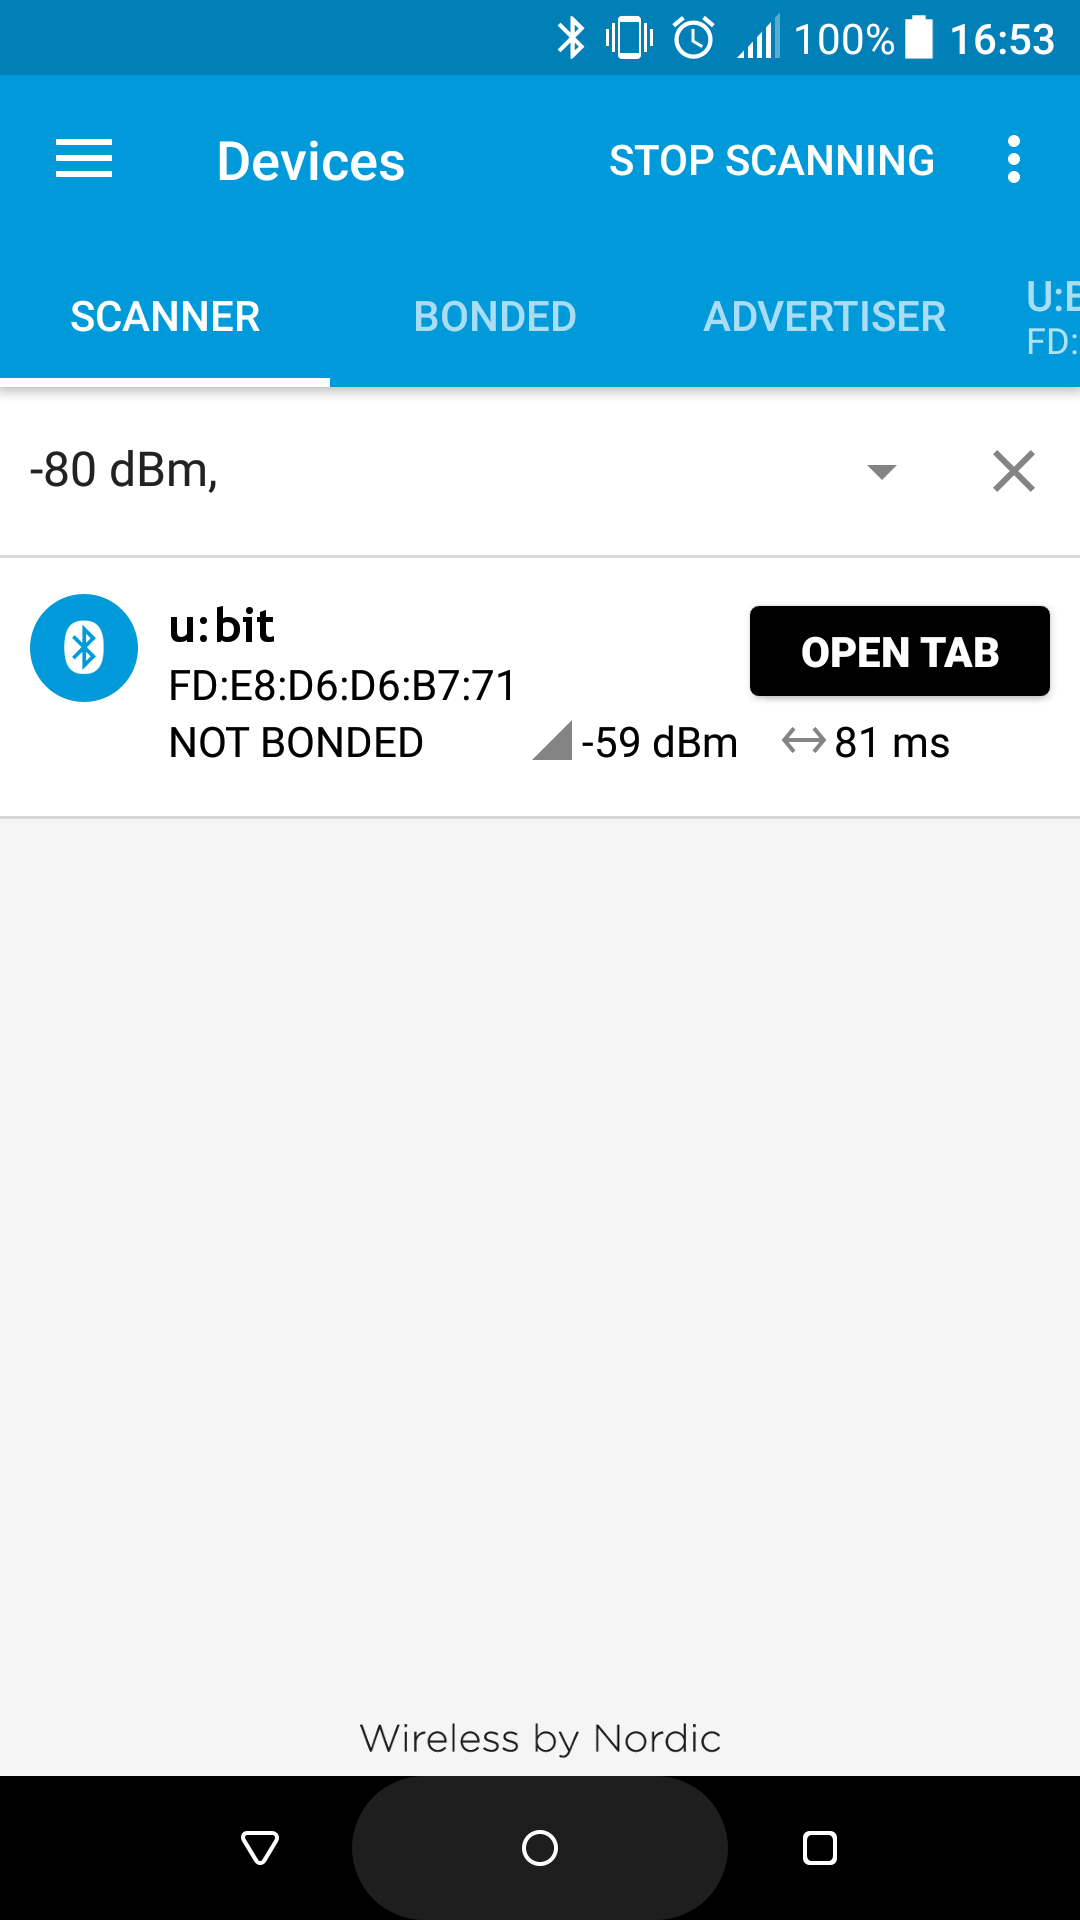
\includegraphics[width=0.9\linewidth]{example_connect_scan.png}
\caption{nRF Connect scan.}
\label{fig::example_scanning}
\end{minipage}%
\begin{minipage}{0.5\linewidth}
\centering
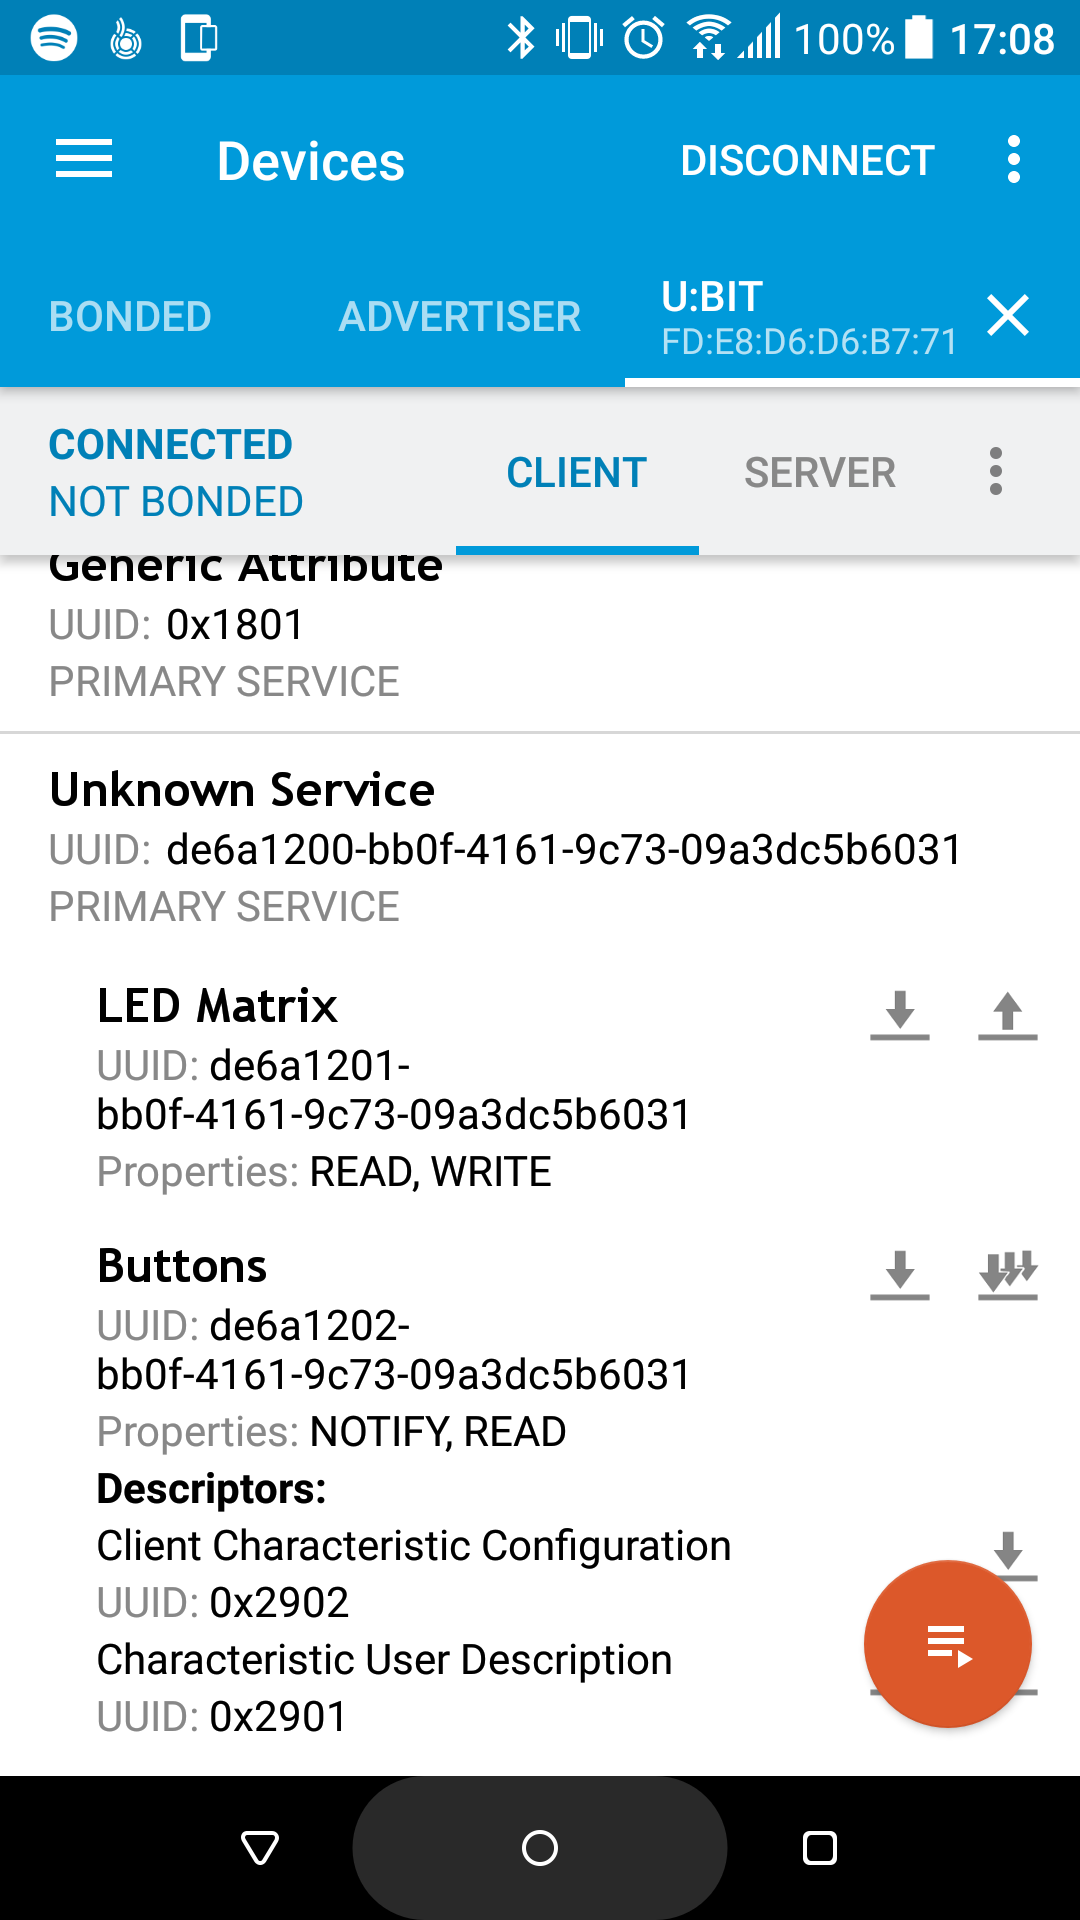
\includegraphics[width=0.9\linewidth]{example_connect_gatt.png}
\caption{Example services.}
\label{fig::example_services}
\end{minipage}
\end{figure}

\newpage
\noindent
\setcounter{section}{0}
\renewcommand{\thesection}{\arabic{section}}
\renewcommand{\thesubsection}{\arabic{section}.\arabic{subsection}}

\section{Heads up}
Bluetooth Low Energy (BLE) is a messy beast to tackle, so it might be smart to skim appendix \ref{app::intro_ble} as you go through this lab assignment. Don't fret if you do not get all the details however - some things are better understood when coded, rather than when read.\\
\\
Finally, an honest word from the author of this assignment: Sometimes, documentation about Bluetooth Low Energy can be a little "Meh". Feeling like there should be an easier way to do Bluetooth is completely normal - just remember to breathe with the stomach, and bite the pillow when the going gets rough.\\
\\
Do enjoy :)

\section{First steps - GAP}
The gatekeeper of Bluetooth is the \textit{Generic Access Profile}. This is the part of Bluetooth that handles broadcasting, discovery, the setting up- and managing connections, as well as negotiating security levels.\\
\\
Although GAP is used to establish connections, GAP itself is connectionless, and pretty simple. The bottom line is this: When advertising, a Bluetooth device sends out an \textit{Advertising Packet} of 31 bytes every advertising interval - which can be anything between $20$ milliseconds and $10.24$ seconds.\\
\\
In addition to this, anyone observing the advertiser can send a \textit{scan request} to the device. Upon receiving such a scan request, the device \textit{may} respond with a \textit{Scan Response Packet}, which is also 31 bytes and can contain different information than the Advertising Packet. Note that the device is not required to respond to scan requests, however.\\
\\
GAP happens entirely on the Bluetooth channels 37, 38, and 39, which are reserved for advertising - as illustrated in figure \ref{fig::bluetooth_spectrum} in appendix \ref{app::intro_ble}. The reason that exactly these channels were chosen for advertising is to avoid most of the interference from WiFi, which is most noticeable on the channels 0-9, 11-20, and 23-32.\\
\\
To make matters a little more interesting, the Bluetooth 4.2 specification specifies 4 different ways a device can advertise. The nuances of this is not terribly important for this course, but they are listed here for the interested:
\begin{itemize}
\item \mintinline{text}{ADV_IND}: "Connectable undirected advertising". This is the regular way to advertise. Any other device can request a scan response or a connection.
\item \mintinline{text}{ADV_DIRECT_IND}: "Connectable directed advertising". This is used to ask a specific central for a connection. The packet is a broadcast packet, but scanners will ignore it if the peer address does not match them. In addition, the advertiser itself will ignore all scan requests.
\item \mintinline{text}{ADV_SCAN_IND}: "Scannable undirected advertising". In this mode, the advertiser will ignore all connection requests, but may respond to scan requests.
\item \mintinline{text}{ADV_NONCONN_IND}: "Non-connectable undirected advertising". This is essentially just an information beacon; the advertiser will ignore all scan- and connection requests, and will simply spew out its own Advertising Packets until the end of time.
\end{itemize}

\subsection{Advertising Packet Format}
Even though the Advertising Packet (and Scan Response Packet) consists of 31 bytes, not all are usable by the application programmer. This is because the packet is subdivided into a number of \textit{AD Structs} - or "Advertising Data Structures". Actually, truth be told, each Advertising Packet may \textit{really} send out 47 bytes over the air each advertising interval, but a lot of this is overhead, as illustrated in figure \ref{fig::pdu_breakdown}. The squares with just numbers in them denote fields that are necessary, but not of direct interest to us.\\
\begin{figure}[ht]
\centering
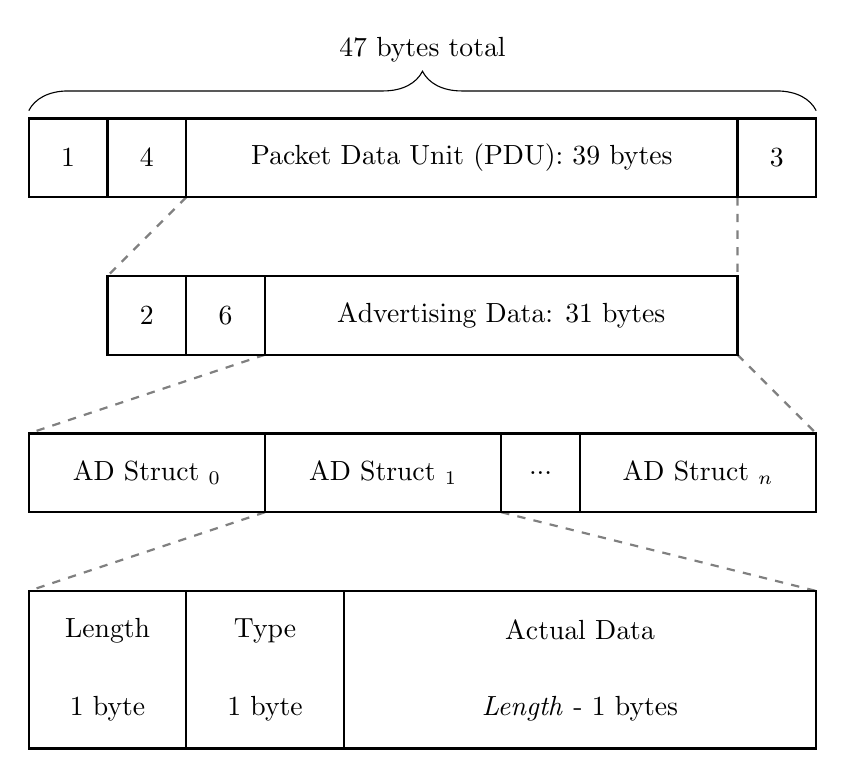
\begin{tikzpicture}
%\draw[gray!35] (0,0) grid (10,-7);
\usetikzlibrary{decorations.pathreplacing}

\draw[decoration={brace,amplitude=5mm}, decorate, yshift=0.1cm] (0,0) -- ++(10,0)
node[midway, above=0.5cm] {47 bytes total};

\draw[gray,dashed,thick] (2,-1) -- +(-1,-1) ++ (7,0) -- ++(0,-1)
++(0,-1) -- +(1,-1) ++(-6,0) -- ++(-3,-1) ++(3,-1) -- +(-3,-1) ++(3,0) -- ++(4,-1);

\draw[thick] (0,0) rectangle ++(1,-1) node[midway] {1}
rectangle ++(1,1)  node[midway] {4} 
rectangle ++(7,-1) node[midway] {Packet Data Unit (PDU): 39 bytes}
rectangle ++(1,1) node[midway] {3};

\draw[thick] (1,-2) rectangle ++(1,-1) node[midway] {2}
rectangle ++(1,1) node[midway] {6}
rectangle ++(6,-1) node[midway] {Advertising Data: 31 bytes};

\draw[thick] (0,-4) rectangle ++(3,-1) node[midway] {AD Struct $_0$}
rectangle ++(3,1) node[midway] {AD Struct $_1$}
rectangle ++(1,-1) node[midway] {...}
rectangle ++(3,1) node[midway] {AD Struct $_n$};

\draw[thick] (0,-6) rectangle ++(2,-2) rectangle ++(2,2) rectangle ++(6,-2);
\path (0,-6) rectangle ++(2,-1) node[midway] {Length}
rectangle ++(2,1) node[midway] {Type}
rectangle ++(6,-1) node[midway] {Actual Data};
\path (0,-7) rectangle ++(2,-1) node[midway] {1 byte}
rectangle ++(2,1) node[midway] {1 byte}
rectangle ++(6,-1) node[midway] {\textit{Length} - 1 bytes};

\end{tikzpicture}
\caption{Breakdown of each GAP advertising transmission unit.}
\label{fig::pdu_breakdown}
\end{figure}\\
Despite the fact that we do not really get to use all the 31 bytes in the advertising data, we must still hand craft the entire field to comply with with the Bluetooth 4.2 spec in our code. In fact, you can see the advertising data used in the example program in listing \ref{code::example_advertise_data}.\\
\begin{listing}[hb]
\begin{minted}{c}
static uint8_t adv_data[] = {
	6, BLE_GAP_AD_TYPE_COMPLETE_LOCAL_NAME,
	'u', ':', 'b', 'i', 't',
	3, BLE_GAP_AD_TYPE_16BIT_SERVICE_UUID_COMPLETE,
	0x0D, 0xF0
};
uint8_t adv_data_length = 11;
\end{minted}
\caption{The advertising data field from the example hex.}
\label{code::example_advertise_data}
\end{listing}\\
Note that the advertising data does not have to use all the 31 bytes available. We are free to use fewer bytes, and therefore transmit less data over the air each advertising interval. This allows us to reduce power consumption a little if we have a really resource constrained application.

\subsection{Write the code}
You have already been handed out some C-files that you may build on. If you happen to be a masochist, you are of course free to discard this code and start from scratch. Otherwise, follow along.\\
\\
In the \mintinline{text}{main} function, you will see a call to \mintinline{text}{bluetooth_init()}. This is simply a wrapper around two calls to first initialize the Nordic SoftDevice, before enabling the Bluetooth Low Energy stack with some sane parameters. You do not need to worry about this; instead, you will be implementing the \mintinline{text}{bluetooth_gap_advertise_start()} function, which is responsible for setting up the AD structs (figure \ref{fig::pdu_breakdown}), and then enabling advertising.\\
\\
The first step is to open up the documentation for the Nordic SoftDevice. Open up \mintinline{text}{softdevice/s130_nrf51_2.0.1_API/html/index.html} in a web browser. From there, navigate to the \mintinline{text}{Modules} tab, then click \mintinline{text}{Generic Access Profile (GAP)}, and then click on \mintinline{text}{Functions}.\\
\\
You will now be greeted with a fairly intimidating looking list of things. If you are feeling a little bit overwhelmed at this point, read section \ref{sec::what_on_earth}. If you are feeling confident, feel free to skip ahead.

\subsubsection{What on earth is all this?}
\label{sec::what_on_earth}
Most of the documentation for the Nordic SoftDevices is handed out as specially formatted comments in the header files of the SoftDevice API. You can then generate a more friendly format, such as an HTML web site, using a handy program called \mintinline{text}{doxygen}. This has already been done for you, but it is pretty easy to do yourselves as well.\\
\\
Doxygen is very handy for integrating documentation into code, and often leads to more up to date documentation in general. The only flip side is that the output is slightly less human friendly than it would otherwise have been, had it been hand crafted by an actual human being. Do not despair though, let us dissect this cryptic output together:

\begin{figure}[h]
\centering
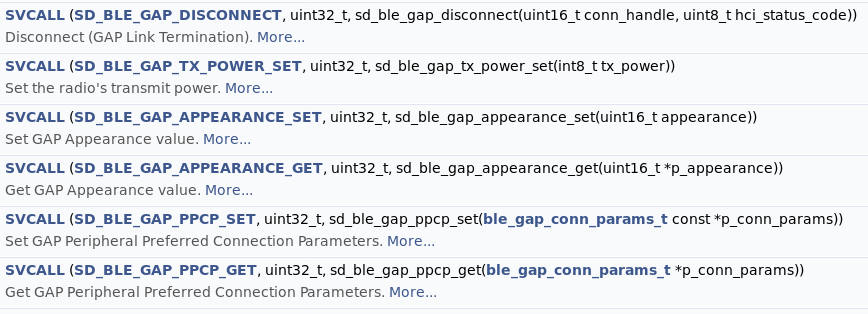
\includegraphics[width=0.9\linewidth]{softdevice_documentation_example.png}
\caption{SoftDevice GAP documentation except.}
\label{fig::gap_documentation_excerpt}
\end{figure}

\noindent
In figure \ref{fig::gap_documentation_excerpt}, you can see an excerpt of the SoftDevice GAP documentation. Each line starts with the macro \mintinline{text}{SVCALL} - which stands for "\mintinline{text}{Supervisor Call}". This is simply an implementation detail, and not something that we have any control over.\\
The actual function that we want to call is listed after this macro. For example, in the line \mintinline{text}{SVCALL(SD_BLE_GAP_TX_POWER_SET, uint32_t [...])}, the function that is available to us is called

\begin{minted}{c}
sd_ble_gap_tx_power_set(int8_t tx_power);
\end{minted}

\noindent
Underneath the \mintinline{text}{SVCALL} line, you can see a short description of what this function does, along with a link that will give you more detailed information about how you should use the function.\\
\\
Many functions will take a pointer to a custom defined struct, instead of several smaller parameters. This is again due to implementation details. In some such cases, the memory that the pointer points to, must remain available after the function has executed. In those cases, manually allocating memory or marking the variable as static is recommended.\\
\\
Finally, it might be worth pointing out some of the coding standard used in the SoftDevice public API:
\begin{enumerate}
\item There is liberal use of the \mintinline{c}{const} keyword, to signal the compiler that a variable should not be changed. This is good practice - especially when dealing with things that can easily break, such as Bluetooth code.
\item Pointer variables are always prefixed with \mintinline{text}{p_}, and in the rare cases of pointer-to-pointer, the prefix \mintinline{text}{pp_} is used. This is heartily recommended, as it is a quick way to kill off some otherwise hard-to-find bugs.
\item In the documentation of each function, the parameters will be marked with either \mintinline{text}{[in]}, \mintinline{text}{[out]}, or \mintinline{text}{[in,out]}. This tells you whether the function intends to modify the input parameter or not. Parameters marked \mintinline{text}{[in]} will not be modified, whereas \mintinline{text}{[out]} and \mintinline{text}{[in,out]} will.
\end{enumerate}

\subsubsection{Set the advertising data}
The first step you need to do is setting the Advertising Packet data content. In the \mintinline{text}{bluetooth.c} file, you will find an incomplete function called \mintinline{text}{bluetooth_gap_advertise_start()}. Your task is to fill out the \mintinline{c}{static uint8_t adv_data[]} array with data according to one or more AD structs, as illustrated in figure \ref{fig::pdu_breakdown}.\\
\\
The function of most interest to you is called \mintinline{text}{sd_ble_gap_adv_data_set}. You are free to skip the Scan Response Packet, in which case you simply set \mintinline{text}{p_sr_data} to \mintinline{c}{NULL}, and \mintinline{text}{srdlen} to \mintinline{c}{0}.\\
\\
For a complete list of the AD Struct types that this SoftDevice supports, you may check out \mintinline{text}{Generic Access Profile (GAP)} $\rightarrow$ \mintinline{text}{Defines} $\rightarrow$ \mintinline{text}{GAP Advertising and Scan Response Data format}.

\warning{If you are interested in using both a complete local name, as well as short local name, there is one caveat you need to be aware of: A short local name must be a continuous subset of the complete local name, starting at the beginning of the complete name - as per the Bluetooth Core Specification Supplement version 7. No worries, it took me ages to figure out as well.}

\subsubsection{Start advertising}
After you have set the advertising data, you need to activate advertising. Check out the documentation for \mintinline{text}{sd_ble_gap_adv_start}. Note that this function call takes a pointer to a \mintinline{text}{ble_gap_adv_params_t} struct.\\
\\
To get the fields of this struct, follow the link in the documentation of the \mintinline{text}{sd_ble_gap_adv_start} function. New tabs for each link you have to follow is advisable, but remember to close the ones you no longer need - otherwise you \textit{will} be overrun with information quickly.\\
\\
Hint: Only the fields \mintinline{text}{type} and \mintinline{text}{interval} are of particular interest, while the rest of the struct can be all zeros. A neat way to do this without manually setting each field is using the \mintinline{c}{memset} function, provided by \mintinline{c}{<string.h>}:

\begin{minted}{c}
ble_gap_adv_params_t adv_params;
memset(&adv_params, 0, sizeof(adv_params));
// Then set only the interesting fields
\end{minted}
To get the documentation for \mintinline{c}{memset}, you may call \mintinline{text}{man 3 memset} in a terminal, but the long and short of it is this: Fill \mintinline{c}{sizeof(adv_params)} number of bytes with all zeros, starting at the address of \mintinline{text}{adv_params}.\\
\\
You stand free to choose the advertising type, but you are most likely interested in using \mintinline{text}{BLE_GAP_ADV_TYPE_ADV_IND}. You can find a complete list of advertising types under \mintinline{text}{Generic Access Profile (GAP)} $\rightarrow$ \mintinline{text}{Defines} $\rightarrow$ \mintinline{text}{GAP Advertising types}.

\subsection{Print to check your code}
All the SoftDevice calls will return 0 (which is the value of\mintinline{text}{NRF_SUCCESS}) upon successful execution. You can print this over UART to the computer by using the provided \mintinline{text}{ubit_uart_print} function - which works the same way \mintinline{text}{printf} does, except that \mintinline{text}{ubit_uart_print} only accepts integers. An example invocation looks like this:
\begin{minted}{c}
ubit_uart_init(); // Call once
ubit_uart_print("My favorite number is %d\n\r", 2);
\end{minted}
To read the micro:bit UART output, you may use any serial terminal program that you choose, with the baudrate 9600. The micro:bit will most likely mount as \mintinline{text}{/dev/ttyACM0}. An example using the \mintinline{text}{picocom} program looks like this:
\begin{minted}{text}
picocom -b 9600 /dev/ttyACM0
\end{minted}
\warning{If you have any other USB UART interfaces connected to the computer, the micro:bit may mount as \mintinline{text}{/dev/ttyACM1} instead. You can call \mintinline{text}{dmesg --follow} and then connect the micro:bit if you want to know for sure where it mounts.}

\subsection{Check with your phone}
If your program compiles and runs, you may check with your phone to see if there is anything on the air. Use the nRF Connect app and start scanning. Your micro:bit should now broadcast its name, along with any other AD Structs that you might have included.\\
\\
If you made it, take a moment to savor your victory; writing Bluetooth Low Energy firmware is not a trivial task ;)\\
\\
Note that if you try to connect to your micro:bit at this point, you will be met with very anticlimactic behavior: The default when a device is attempted connected to, is to stop advertising. However, since we have not implemented any connection acceptance yet, the device will simply turn off advertising and then idle - and then your phone will time out.\\
\\
Finally, you might have noticed that the nRF Connect app reports a different advertising interval than you specified. For example, if you chose 80 ms in your code, you will typically see an actual advertising interval of around 85 ms. This is because the Bluetooth spec will add a random delay to the specified interval, in order to reduce the likelihood of packet collisions.

\section{Get your game on - GATT}
GAP is cool and all, but the real workhorse of Bluetooth is the GATT; the \textit{Generic Attribute Profile}. Unlike the GAP, which only deals with details regarding interactions between devices, the GATT deals with data transfer.\\
\\
Since Bluetooth 4.1, it became possible to use the mysterious L2CAP (the \textit{Logical Link Controller and Adaptation Protocol}) for higher throughput connection-oriented data transfer channels. Thus, you \textit{could} use this layer for your data transfer directly. Nevertheless, at the time of writing, Bluetooth data transfer seems synonymous with GATT usage in some shape or form. For those interested, the Bluetooth Low Energy layers are illustrated in figure \ref{fig::bluetooth_stack_differences}.\\
\\
It is perfectly normal to be confused about GAP and GATT at this point, but the essence is this: GAP takes care of advertising, connections and security. GATT is a \textit{profile} that uses a \textit{protocol} named ATT (Attribute Protocol). Through a set of black magic, the GATT uses the ATT to provide a means for data transfer.

\subsection{Protocols and Profiles}
It is useful to have at least a high-level understanding of what the Bluetooth spec talks about when it discusses protocols and profiles. Still, a deep knowledge about these things should not be necessary to use Bluetooth Low Energy, so please do not fret if some of the concepts remain fuzzy.

\subsubsection{Protocols}
In Bluetooth, a \textit{protocol} is a layer that implements low-level details like packet formatting, routing, encoding, multiplexing, and some interface that allows data to be sent between peers.\\
\\
The ATT (Attribute protocol) is an example of a protocol. The ATT does not have that much to it; it is merely a simple client-server stateless way to exchange data, presented as so-called "attributes". A Bluetooth device can be either a client, a server, or both - regardless of whether it is a master or a slave.\\
\\
Inside the ATT, you find a set of attributes. Each attribute is a collection of four components:
\begin{enumerate}
\item A 16-bit attribute handle.
\item A number known as a Universally Unique Identifier (UUID).
\item A set of read- and write permissions.
\item The value, or the real data of the attribute.
\end{enumerate}
Each time a client wants to read- or write an attribute value, it issues a request to the ATT server. The server must then fully process this single request, before tending to any other requests.\\
\\
When a client accesses an attribute, it uses the 16-bit attribute handle to identify which attribute it is trying to access. The UUID is a 128-bit (16 byte) number that describes the type or nature of the attribute data. When reading, the serves does minimal checking; the client is responsible for interpreting and understanding the supplied data. This is unlike a write operation - which the server is free to reject if the client data does not fit the expected format.

\subsubsection{Profiles}
A \textit{profile} is a recipe for how to use one or more protocols to serve a certain purpose, and achieve a particular goal. An example of such a profile is the GATT, or the Generic Attribute Profile.\\
\\
The GATT heavily relies on the ATT, but to further convolute matters more, the GATT introduces some new concepts and terminology. The most important difference the GATT introduces is data organization. In GATT, data is ordered in a hierarchy of so-called \textit{services}. A service is a collection of \textit{characteristics}, and a set of relationships to other services. Characteristics are just conceptually similar pieces of data grouped together. See figure \ref{fig::gatt_server_service_characteristic} for an illustration of this.
\begin{figure}[h]
\centering
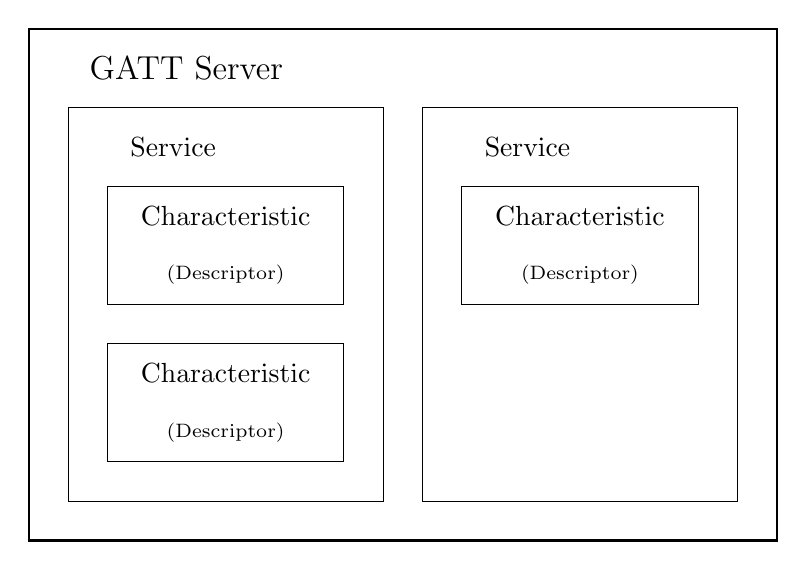
\begin{tikzpicture}

\draw[thick] (-0.5,-0.5) rectangle ++(9.5,6.5);
\path (0,6) rectangle ++(3,-1) node[midway] {\large GATT Server};


\draw (0,0) rectangle ++(4, 5);
\path (0.5,5) rectangle ++(3,-1) node[midway,left] {Service};

\draw (0.5,0.5) rectangle ++(3,1.5);
\path (0.5, 2) rectangle ++(3,-0.75) node[midway] {Characteristic};
\path (0.5, 0.5) rectangle ++(3,0.75) node[midway] {\scriptsize(Descriptor)};

\begin{scope}[yshift=2cm]
\draw (0.5,0.5) rectangle ++(3,1.5);
\path (0.5, 2) rectangle ++(3,-0.75) node[midway] {Characteristic};
\path (0.5, 0.5) rectangle ++(3,0.75) node[midway] {\scriptsize(Descriptor)};
\end{scope}

\begin{scope}[xshift=4.5cm]
\draw (0,0) rectangle ++(4, 5);
\path (0.5,5) rectangle ++(3,-1) node[midway,left] {Service};

\begin{scope}[yshift=2cm]
\draw (0.5,0.5) rectangle ++(3,1.5);
\path (0.5, 2) rectangle ++(3,-0.75) node[midway] {Characteristic};
\path (0.5, 0.5) rectangle ++(3,0.75) node[midway] {\scriptsize(Descriptor)};
\end{scope}
\end{scope}

\end{tikzpicture}
\caption{Conceptual illustration of a GATT server.}
\label{fig::gatt_server_service_characteristic}
\end{figure}
\\
If you have a background in object-oriented programming, it might be helpful to think of services as \textit{classes}, and characteristics as \textit{member variables}.
\\
\\
\warning{The Bluetooth spec might have gone a \textit{little} overboard with all the abbreviations. Remember to breathe with the stomach as you take it all in.}

\subsection{Create a Service}
As you can probably guess from figure \ref{fig::gatt_server_service_characteristic}, the first thing we want to do to make GATT useful is to add a Service. Before we do this, we need to do some housekeeping; first off, include "\mintinline{text}{ble_gatts.h}". Secondly, we need to allocate some persistent memory that can keep track of our new service. We can do this by creating a \mintinline{c}{static} struct at the top of \mintinline{text}{bluetooth.c}, like so:

\begin{minted}{c}
static struct {
	uint16_t conn_handle;
	uint16_t service_handle;
	ble_gatts_char_handles_t matrix_handles;
} m_service_ubit;
\end{minted}
This struct might look cryptic, but it is merely a representation of a - "Service (\mintinline{c}{m_service_ubit}), which has a single "Characteristic" (\mintinline{c}{matrix_handles}). The reason for the \mintinline{text}{_m} prefix on \mintinline{c}{m_service_ubit} is simply to denote to ourselves that this variable is reachable in the whole \textbf{m}odule. Getting into the habit of using simple prefixes like this is a very neat way of doing some simple sanity checks .\\
\\
This is well and nice, but we still need to hold our horses a bit. Before we can actually add the service and characteristic, we need to give it some sort of ID, so the Bluetooth Stack knows how to address it. This is done by adding a new entry to the SoftDevice UUID table.

\subsubsection{Add a Vendor Specific UUID}
The Bluetooth spec defines a set of 16 bit UUIDs for the members of the Bluetooth Special Interest group, and some widely adopted services. Sadly, we are not on this list, so we need to create our own, longer, 128 bit UUID and use that instead.\\
\\
In a terminal, call \mintinline{text}{uuidgen}. You will get a random string of hexadecimal values, for example "\mintinline{text}{d8ff10af-2e1a-4bcf-b479-7f43a6995846}". This is now our base UUID, that we will supply to the SoftDevice.\\
\\
Since the \mintinline{text}{uuidgen} command yields a UUID in big endian, and the SoftDevice represents UUIDs in little endian, we technically have to enter our UUID in reverse. For the UUID above, you would enter this in \mintinline{text}{bluetooth.c}:
\begin{minted}{c}
#define CUSTOM_UUID_BASE {{\
 0x46, 0x58, 0x99, 0xa6, 0x43, 0x7f, 0x79, 0xb4,\
 0xcf, 0x4b, 0x1a, 0x2e, 0xaf, 0x10, 0xff, 0xd8\
}}
\end{minted}
In this specific case, it would not matter if you entered the UUID the wrong way, since this would simply correspond to a different randomly generated UUID. However, it would matter if you were implementing a "known and registered" service, so it is good to get into the habit of doing it correctly.\\
\\
Since we will be implementing a single service with a single characteristic, we will need two more UUIDs after we have our base; one for the service, and one for the characteristic. Instead of specifying a full 128-bit UUID for these however, we simply need to supply two 16-bit "modifiers" to the base UUID. In this example, we are going to create a service called "\mintinline{text}{ubit}", with a characteristic called "\mintinline{text}{matrix}", so add the following to \mintinline{text}{bluetooth.c}:
\begin{minted}{c}
#define CUSTOM_UUID_SERVICE_UBIT 0xdead
#define CUSTOM_UUID_CHAR_MATRIX 0xbabe
\end{minted}
Since we are using "vendor specific" UUIDs, the actual values of the modifiers \mintinline{text}{CUSTOM_UUID_SERVICE_UBIT} and \mintinline{text}{CUSTOM_UUID_CHAR_MATRIX} are not important, and you are free to set them to any 16-bit number of your liking, as long as they are not identical.\\
\\
Now that we have decided what our UUIDs, will be, we must also tell this to the SoftDevice. In \mintinline{c}{bluetooth_gatts_start()}, you do this by running the following code:
\begin{minted}{c}
ble_uuid128_t base_uuid = CUSTOM_UUID_BASE;

ble_uuid_t ubit_service_uuid;
ubit_service_uuid.uuid = CUSTOM_UUID_SERVICE_UBIT;

err_code = sd_ble_uuid_vs_add(
	&base_uuid,
	&ubit_service_uuid.type
);
\end{minted}
This is all well and fine. We have now added our own vendor specific service UUID to the SoftDevice UUID table. The only catch is of course that we have not added the actual service yet. No reason for despair though, we will do that next.

\subsubsection{Add a Service to our UUID}
We already have space for our service, namely \mintinline{c}{m_service_ubit}, that we declared earlier. Now we will tell the SoftDevice that this is what we intend to use for the service itself. Look into the \mintinline{c}{sd_ble_gatts_service_add} function, which you can find documentation for under \mintinline{text}{Generic Attribute Profile (GATT) Server} $\rightarrow$ \mintinline{text}{Functions}.\\
\\
The type of the service should be primary. The \mintinline{text}{p_uuid} parameter should be a pointer to our service UUID. Finally, the \mintinline{text}{p_handle} parameter should be a pointer to the \mintinline{text}{service_handle} member of \mintinline{text}{m_service_ubit}.\\
\\
It is probably smart to check that this call returns \mintinline{text}{NRF_SUCCESS} (defined to be 0) before moving on.

\subsubsection{Add the Characteristic UUID}
Now that we have added our service UUID and defined a handle for it, we need to populate that service with a characteristic. The first step is of course adding the UUID for our characteristic. This is done the same way as before:
\begin{minted}{c}
ble_uuid_t matrix_uuid;
matrix_uuid.uuid = CUSTOM_UUID_CHAR_MATRIX;

err_code = sd_ble_uuid_vs_add(
	&base_uuid,
	&matrix_uuid.type
);
\end{minted}

\subsubsection{Add the Characteristic}
A quick inventory check of what we have done so far: First off, we added our own vendor specific service UUID. Then we added the actual service to the SoftDevice. Now we have added a characteristic UUID to that service, but we have yet to add the "meat" of the characteristic itself. This is done by using the \mintinline{text}{sd_ble_gatts_characteristic_add} function, so if you are feeling adventurous, feel free to just read the documentation for that call and get going. Otherwise, read on.\\
\\
\warning{The upcoming steps will probably seem completely arbitrary unless you have used a similar API before. Trust me, after a few times it starts making sense :)}\\
\\
A characteristic consists of zero or more \textit{descriptors}, a set of \textit{characteristic metadata}, and some \textit{attribute metadata}. You can be pretty sure we have to deal with all of these. It is very easy to get lost in the process of setting this up, so I will not force you to do it completely on your own - still, you are encouraged to check out the documentation and try to understand what we are doing as you follow along.\\
\\
First, we are going to set up the characteristic metadata, as such:
\begin{minted}{c}
static uint8_t matrix_char_desc[] = {
	'L', 'E', 'D', ' ', 'M', 'a', 't', 'r', 'i', 'x'
};
ble_gatts_char_md_t matrix_char_md;
memset(&matrix_char_md, 0, sizeof(matrix_char_md));
matrix_char_md.char_props.read = 1;
matrix_char_md.char_props.write = 1;
matrix_char_md.p_char_user_desc = matrix_char_desc;
matrix_char_md.char_user_desc_max_size = 10;
matrix_char_md.char_user_desc_size = 10;
\end{minted}
You can probably interpret most of this yourself. We create a characteristic that is both read- and writable. Then we describe the characteristic by adding the descriptor "\mintinline{text}{LED Matrix}", which is a UTF-8 encoded string that is not null-terminated. Since the string should not be terminated by a \mintinline{text}{NULL}, we have to supply the SoftDevice with the length of the descriptor as well. Some descriptors are allowed to be changed during operation, so we also supply a max length. In this case, we do not want the descriptor to be mutable, so we leave the \textit{descriptor metadata} (\mintinline{text}{p_user_desc_md}) unset. You can see the documentation for the whole characteristic metadata struct by going to \mintinline{text}{Generic Attribute Profile (GATT) Server} $\rightarrow$ \mintinline{text}{Structures} $\rightarrow$ \mintinline{text}{ble_gatts_char_md_t}.\\
\\
Next up is making the attribute that our characteristic will refer to. Remember that GATT uses ATT behind the scenes, so it probably does not come as a surprise that we have to set some attribute metadata as well:
\begin{minted}{c}
ble_gatts_attr_md_t matrix_attr_md;
memset(&matrix_attr_md, 0, sizeof(matrix_attr_md));
matrix_attr_md.read_perm.lv = 1;
matrix_attr_md.read_perm.sm = 1;
matrix_attr_md.write_perm.lv = 1;
matrix_attr_md.write_perm.sm = 1;
matrix_attr_md.vloc = BLE_GATTS_VLOC_USER;
\end{minted}
Here, we are specifying the access restrictions to our attribute in the ATT server. The magic values for \mintinline{text}{lv} and \mintinline{text}{sm} set the \textit{Security Mode} and \textit{Level} of authentication needed to modify the attribute. When both are 1, we have an open link, so no security is needed. Even though this assignment will not touch on the security aspects of Bluetooth Low Energy, the Bluetooth spec boasts an impressive set of security considerations, like signing, encryption, and man-in-the-middle-attack protection.\\
In addition to setting the access restrictions for our attribute, we also tell the SoftDevice where the attribute value resides, that is, the \textbf{v}alue \textbf{loc}ation of the attribute. The value \mintinline{text}{BLE_GATTS_VLOC_USER} means that the user (us) is responsible for ensuring that the attribute value is always stored in a valid location throughout the entire lifetime of the attribute. We will tend to this next.\\
\\
Finally, we can create the attribute value. This needs to be reachable in the entire module, so add \mintinline{c}{static uint8_t m_matrix_attr_value = 0;} to the top of \mintinline{text}{bluetooth.c}. After that, we simply have to put this value and the metadata variables together, like so:
\begin{minted}{c}
ble_gatts_attr_t matrix_attr;
memset(&matrix_attr, 0, sizeof(matrix_attr));
matrix_attr.p_uuid = &matrix_uuid;
matrix_attr.p_attr_md = &matrix_attr_md;
matrix_attr.init_len = 1;
matrix_attr.max_len = 1;
matrix_attr.p_value = &m_matrix_attr_value;
\end{minted}
And then, to register our beautiful creation with our SoftDevice overlord, we call \mintinline{text}{sd_ble_gatts_characteristic_add}:
\begin{minted}{c}
err_code = sd_ble_gatts_characteristic_add(
	m_service_ubit.service_handle,
	&matrix_char_md,
	&matrix_attr,
	&m_service_ubit.matrix_handles
);
\end{minted}
Congratulations, your Bluetooth application is now approximately 100\% cooler than before. However, it is still not connectable. We need to fix that, so read on.

\section{Serve connections}
We are nearly there. All that remains is to react to \textit{connection events} and update the \textit{connection handle} in out service. In the general case, you have to set up an event buffer, fill it up with incoming events, and process each of them in order.\\
\\
In your case, this is already done for you. At the bottom of your \mintinline{text}{main} function, simply call \mintinline{text}{bluetooth_serve_forever()}.\\
\\
If you inspect that function, you will see that all it essentially does, is listen for \mintinline{text}{BLE_GAP_EVT_CONNECTED} and \mintinline{text}{BLE_GAP_EVT_DISCONNECTED}. You can probably guess that these signify connection requests and disconnects through GAP. When these happen, we update the connection handle in our service accordingly.\\
\\
In addition to this, the infinite loop in \mintinline{text}{bluetooth_serve_forever} sets and clears the LED matrix on the micro:bit according to the value of our characteristic.\\
\\
\warning{Do not forget to initialize the LED matrix before calling \mintinline{text}{bluetooth_serve_forever}. Find an appropriate place to call the init function.}

\section{Instant gratification}
You may now compile and flash your code. On your phone, you should now see something similar to figure \ref{fig::exercise_scanning} when you scan. If you try to connect, you should get something akin to figure \ref{fig::exercise_service}. Note that we are able to use Unicode letters (encoded as UTF-8) in the GAP advertising packet, as seen in figure \ref{fig::exercise_scanning} with the umlaut \textit{ü}. Even so, the nRF Connect app does not support all Unicode letters, so some of the more esoteric glyphs might cause the app to ignore your advertising packet.\\
\\
Also note that we can recognize the UUID modifiers that we chose for the service and characteristic, as seen highlighted in figure \ref{fig::exercise_service}.\\
\\
\begin{figure}[ht]
\centering
\begin{minipage}{0.5\linewidth}
\centering
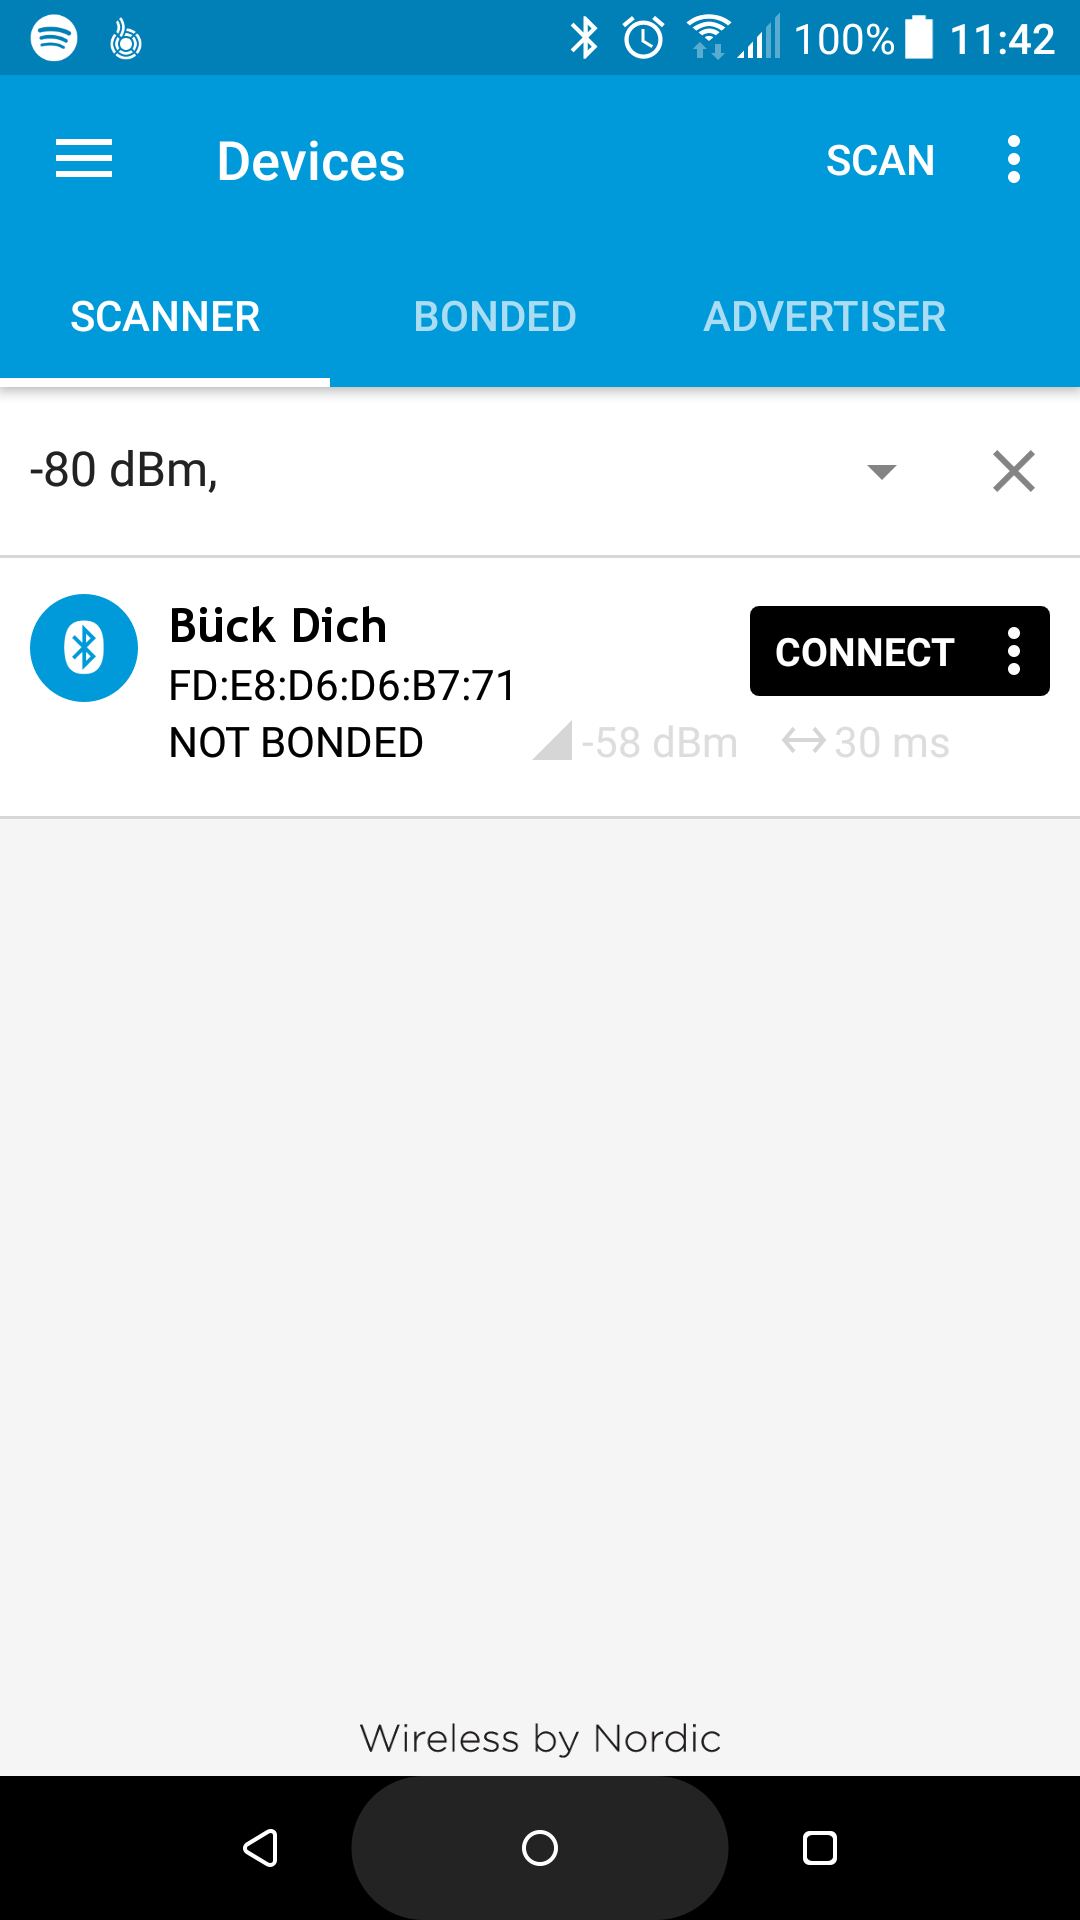
\includegraphics[width=0.9\linewidth]{example_exercise_scan.png}
\caption{nRF Connect scan.}
\label{fig::exercise_scanning}
\end{minipage}%
\begin{minipage}{0.5\linewidth}
\centering
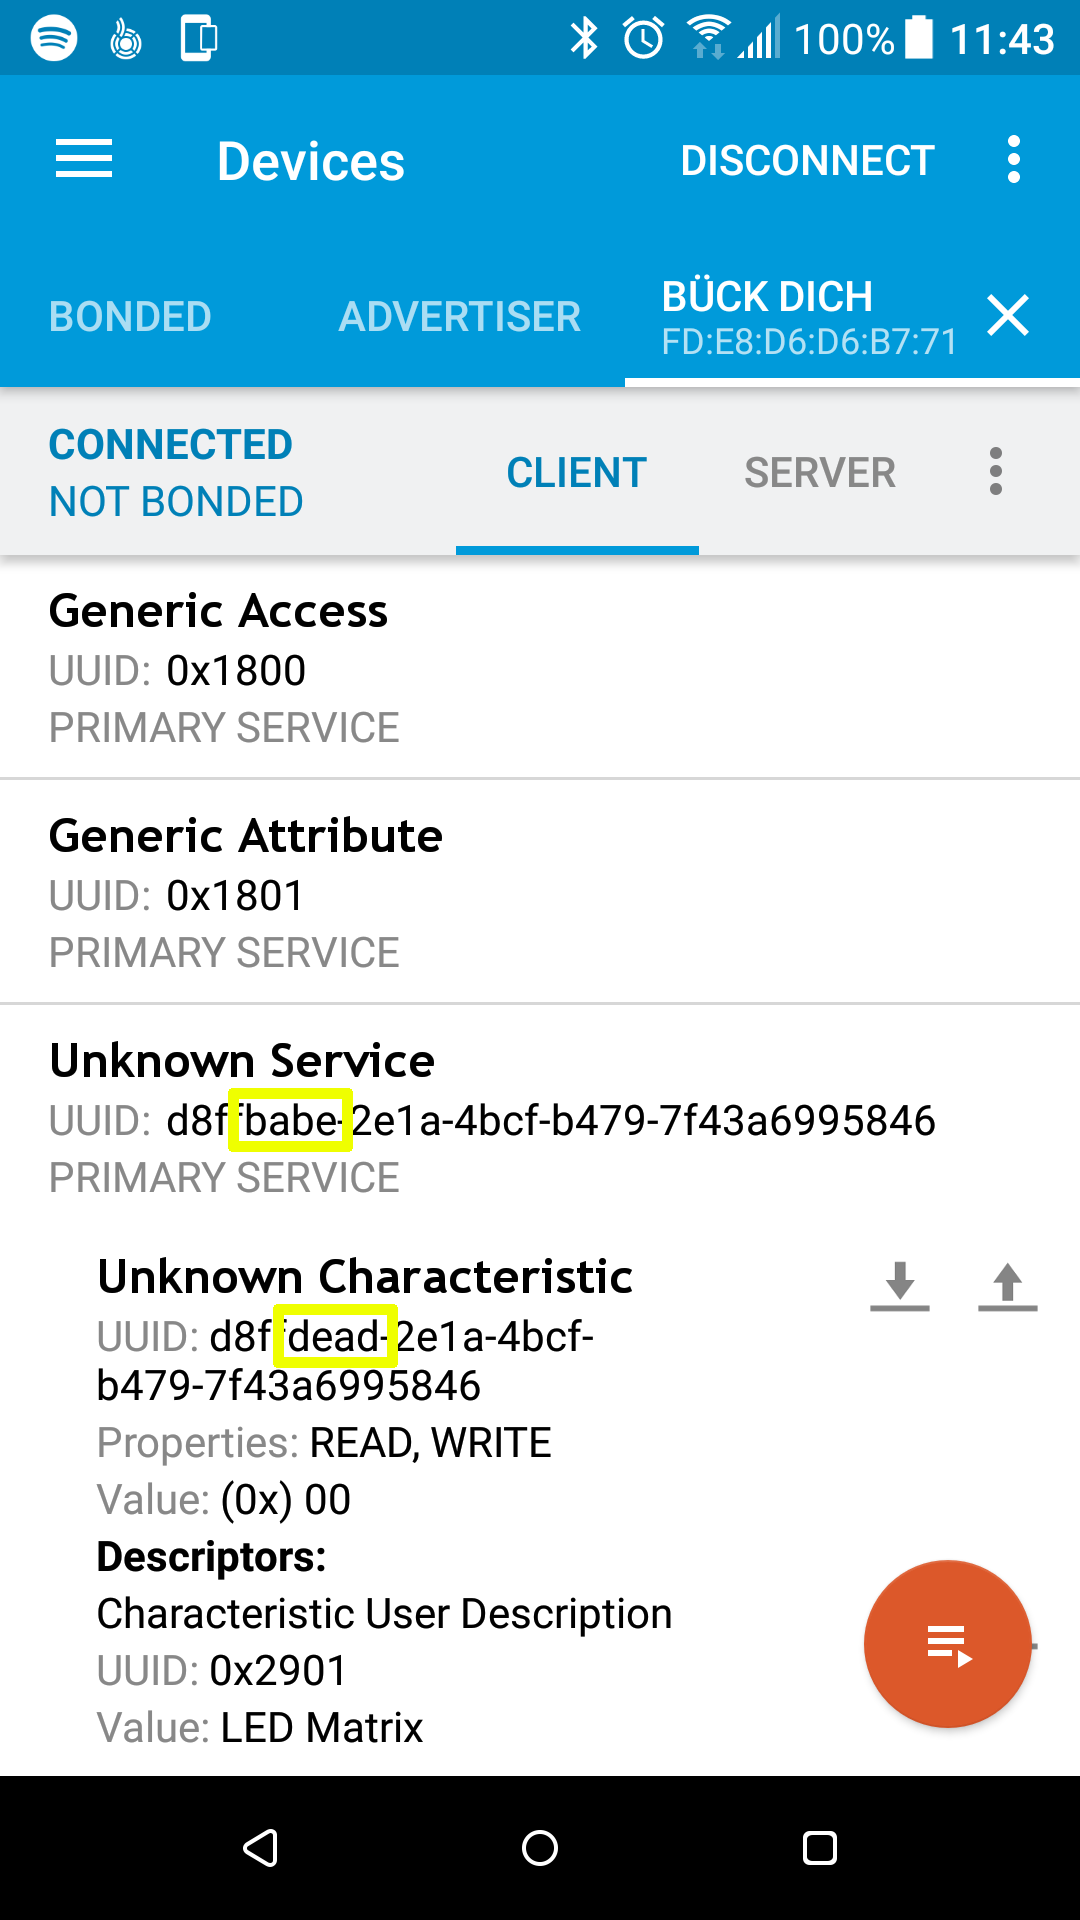
\includegraphics[width=0.9\linewidth]{example_exercise_gatt_highlighted.png}
\caption{Custom service.}
\label{fig::exercise_service}
\end{minipage}
\end{figure}\noindent
You can now download the Characteristic User Description descriptor by clicking the download symbol underneath the descriptors category in figure \ref{fig::exercise_service}. The descriptor then tells you that this is a characteristic for the LED matrix.\\
\\
As in the example program, you can toggle the LED matrix by writing a byte to the matrix characteristic.

\section{What now?}
Now you are free to integrate the micro:bit into your project however you wish, for example by broadcasting the score over Bluetooth to your phone. The remainder of this section will mainly deal with two things; firstly, I will give some tips on how to add notification support, so you do not have to manually read a characteristic when it changes. Secondly, I will give a few suggestions about how you can interface the micro:bit with the rest of your project.

\subsection{Notifications}
Suppose you want to add notifications for when you press buttons on the micro:bit. This can be done by either adding a new service, or adding a new characteristic to our already existing service. Since our service is named "ubit" and deals with the micro:bit hardware, it makes the most sense to expand this service.\\
\\
The first thing you would do, is to add new handles for the new service, by updating the definition of \mintinline{text}{m_service_ubit}:
\begin{minted}{c}
static struct {
	uint16_t conn_handle;
	uint16_t service_handle;
	ble_gatts_char_handles_t matrix_handles;
	ble_gatts_char_handles_t button_handles;
} m_service_ubit;
\end{minted}
Since we have two buttons on the micro:bit, it makes sense to use an array of two \mintinline{c}{uint8_t}s to represent their state - though you stand free to squeeze them both into one byte, if you want to be greedy with the resources:
\begin{minted}{c}
static uint8_t m_button_press_a_b[2] = {0, 0};
static uint8_t m_button_press_a_b_previous[2] = {0, 0};
\end{minted}
This is analogous to our \mintinline{c}{static uint8_t m_matrix_attr_value} from earlier. The reason we create two copies, is so we can notify the phone only when the button states update. This way, we do not needlessly transmit the button states unless they have changed since the last time we transmitted.\\
\\
Adding the rest of the characteristic is similar to how we added the LED matrix characteristic, with some minor tweaks. The most obvious is that we do not want to make the attribute writable, so the attribute metadata will look like this instead:
\begin{minted}{c}
ble_gatts_attr_md_t button_attr_md;
memset(&button_attr_md, 0, sizeof(button_attr_md));
button_attr_md.vloc = BLE_GATTS_VLOC_USER;
button_attr_md.read_perm.sm = 1;
button_attr_md.read_perm.lv = 1;
\end{minted}
Next, we have to make sure the characteristic metadata matches the attribute metadata. There is one catch though; since the client (the phone) should be able to subscribe and unsubscribe to notifications, we need another piece of metadata describing whether the client wants notifications or not. This is stored in the Client Characteristic Configuration Descriptor, or the aptly named CCCD. The Bluetooth Special Interest Group dodged a bullet by not naming it the Client Characteristic Configuration Property.\\
\\
This descriptor is managed by the SoftDevice, so we should allocate it to the stack, rather than to user memory. After that, we need to tell the characteristic metadata to use the CCCD. Do not lose hope if this sounds like made-up gibberish; it should look like this:
\begin{minted}{c}
ble_gatts_attr_md_t button_cccd_md;
memset(&button_cccd_md, 0, sizeof(button_cccd_md));
button_cccd_md.vloc = BLE_GATTS_VLOC_STACK;
button_cccd_md.read_perm.lv = 1;
button_cccd_md.read_perm.sm = 1;
button_cccd_md.write_perm.lv = 1;
button_cccd_md.write_perm.sm = 1;

static uint8_t button_char_desc[] = {
	'B', 'u', 't', 't', 'o', 'n', 's'
};
ble_gatts_char_md_t button_char_md;
memset(&button_char_md, 0, sizeof(button_char_md));
button_char_md.char_props.read = 1;
button_char_md.char_props.notify = 1;
button_char_md.p_char_user_desc = button_char_desc;
button_char_md.char_user_desc_max_size = 7;
button_char_md.char_user_desc_size = 7;
button_char_md.p_cccd_md = &button_cccd_md;
\end{minted}
If you fill out the rest of the characteristic, and then add it to the SoftDevice by calling \mintinline{text}{sd_ble_gatts_characteristic_add}, you will see a new characteristic when you connect to the micro:bit (you might have to go to settings and "Refresh services" in the nRF Connect app). Still, the characteristic will not do anything, since we never update the button attribute value. This is next on our list.

\subsubsection{Updating the client}
To send notifications, we need to use the function \mintinline{text}{sd_ble_gatts_hvx}. HVX stands for "Handle Value X". I think we can all agree that the price for best function name does not go to \mintinline{text}{sd_ble_gatts_hvx}. Either way, here you can see an example invocation that transmits the state of our buttons:
\begin{minted}{c}
if(m_service_ubit.conn_handle != BLE_CONN_HANDLE_INVALID){
	uint16_t notification_length = 2;
	
	ble_gatts_hvx_params_t hvx_params;
	memset(&hvx_params, 0, sizeof(hvx_params));
	hvx_params.handle = m_service_ubit.button_handles.value_handle;
	hvx_params.type = BLE_GATT_HVX_NOTIFICATION;
	hvx_params.p_len = &notification_length;
	hvx_params.p_data = m_button_press_a_b;
	
	sd_ble_gatts_hvx(
		m_service_ubit.conn_handle,
		&hvx_params
	);
}
\end{minted}
You would call this at the bottom of the infinite loop in \mintinline{text}{bluetooth_serve_forever}. Transmitting only when the button state has changed is simply a matter of comparing \mintinline{text}{m_button_press_a_b} and \mintinline{text}{m_button_press_a_b_previous}. This is up to you.\\
\\
If you implement all this, you have essentially replicated the example program that was handed out, congratulations!

\subsection{Interfacing to the rest of the project}
When interfacing with the rest of your project, there is several ways to approach the problem. The two ways that I find most obvious are described here.

\subsubsection{Direct connection}
When interfacing with the rest of your project, there is several ways to approach the problem. The micro:bit supports both SPI and I$^2$C (aka TWI), as well as UART. It is thus possible to connect the micro:bit to either node 1 or node 2, and interface it using one of the above protocols.\\
\\
\warning{The micro:bit runs on 3.3V, while the rest of the project runs on 5V. Get a logic level converter, or a set of high frequency optocouplers if you want to follow this approach.}\\
\\
This would also require you to write your own SPI or I$^2$C drivers. For those of you who have taken TTK4235, this should be a cake walk.

\subsubsection{Indirect connection}
Another approach is to simply use the host computer as a middle man. You may then use the micro:bit to communicate with the computer, which will in turn communicate with one of the nodes in your project.\\
\\
This would require you to extend the UART driver for the micro:bit to also support receiving messages, as the driver handed out is only unidirectional. It would also require you to write a bridging program running on the computer. This bridging program simply has to forward messages between two serial ports. Considering the myriad of serial libraries out there, this task should be dirt simple - for example pySerial for Python, Nerves for Elixir, SerialPort for Ruby, etc.

\subsubsection{Conclusion}
If you want to interface the micro:bit with the rest of your project using either of these methods, the amount of work should roughly be the same.\\
\\
Using a direct connection removes the need for a man-in-the-middle, but it places more emphasis on hardware, as you have to correctly convert the logical levels in order to not damage the micro:bit.\\
\\
Using the computer as a middle man, there is no extra hardware requirements at all, and the problem is reduced to "simply" writing correct code. In conclusion, it depends on what you are most comfortable working with ;)

\newpage
\noindent
\appendix
\section{Introduction to BLE}
\label{app::intro_ble}
Bluetooth Low Energy, or Bluetooth 4.2 is a version of Bluetooth specifically tailored toward low energy applications, as the name suggests. The first version of BLE (Bluetooth 4.0) saw the light of day in 2010, and since then, BLE has had an adoption rate unparalleled by most other technologies. The most influential factor is likely the cellphone market, helped along by the kin of Samsung and Apple. In addition to this, BLE allows for anyone who wants to use it to tweak it their purposes, while still being able to take advantage of the BLE framework. This is in contrast to Bluetooth Classic, which is only focused on a narrow set of pre-defined use cases.\\
\\
Interestingly, in the pursuit of lower power consumption, BLE has scaled back on the punch it packs in terms of data throughput. While you should be comfortably able to listen to music over Bluetooth Classic, this is in reality close to impossible over Bluetooth Low Energy.\\
\\
Even though the radio modulation rate of BLE is 1 Mbps, the protocol itself introduces a lot of overhead. In our case, the nRF51822 can transmit up to 6 data packets par \textit{connection interval} - where a connection interval is simply one data exchange between two devices. Each data packet can contain up to 20 user defined bytes. The shortest possible connection interval is 7.5 ms, and so we are already at a theoretical upper limit of
$$\frac{6 \cdot 20 \cdot 8\ \mathrm{bits}}{7.5\ \mathrm{ms}} = 128\ \mathrm{kbit}/\mathrm{s}$$
Add to that the fact that Bluetooth Low Energy will always try to retransmit lost packages, collisions might happen, the radio might be busy, as so on and so forth. In practice, you can expect to see around 40-80 kbps. This is pretty unimpressive in term of raw data throughput, but Bluetooth Low Energy still shines in what it was intended to be good at, namely low power consumption in resource constrained environments.\\
\\
From a technical point of view, the Bluetooth stack itself has changed over the years. So much so that a Bluetooth Classic cannot talk directly to Bluetooth Low Energy. The different layers of the Bluetooth Classic and Bluetooth Low Energy stacks are illustrated in figure \ref{fig::bluetooth_stack_differences}. Bluetooth Classic is also often called "BR/EDR", which stands for "Basic Rate/Enhanced Data Rate".\\
\\
\begin{figure}[hbt]
\centering
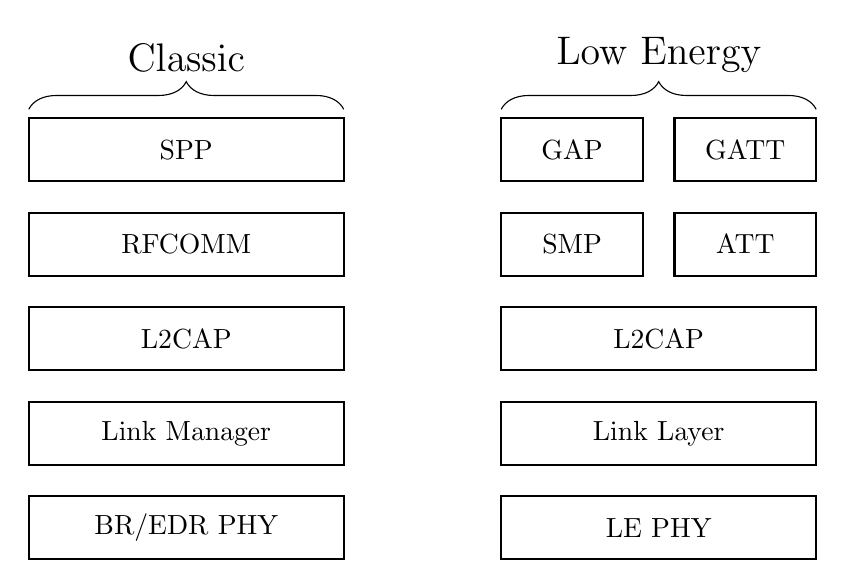
\begin{tikzpicture}[yscale=0.8]
\usetikzlibrary{decorations.pathreplacing}

\draw[thick] (0,0) rectangle ++(4,1) node[midway] {BR/EDR PHY};
\draw[thick] (0,1.5) rectangle ++(4,1) node[midway] {Link Manager};
\draw[thick] (0,3) rectangle ++(4,1) node[midway] {L2CAP};
\draw[thick] (0,4.5) rectangle ++(4,1) node[midway] {RFCOMM};
\draw[thick] (0,6) rectangle ++(4,1) node[midway] {SPP};
\draw[decorate,decoration={brace,amplitude=10pt},yshift=4pt] (0,7) -- ++(4,0) node[midway,above=10pt] {\Large Classic};

\begin{scope}[xshift=6cm]
\draw[thick] (0,0) rectangle ++(4,1) node[midway] {LE PHY};
\draw[thick] (0,1.5) rectangle ++(4,1) node[midway] {Link Layer};
\draw[thick] (0,3) rectangle ++(4,1) node[midway] {L2CAP};
\draw[thick] (0,4.5) rectangle ++(1.8,1) node[midway] {SMP};
\draw[thick] (4,4.5) rectangle ++(-1.8,1) node[midway] {ATT};
\draw[thick] (0,6) rectangle ++(1.8,1) node[midway] {GAP};
\draw[thick] (4,6) rectangle ++(-1.8,1) node[midway] {GATT};
\draw[decorate,decoration={brace,amplitude=10pt},yshift=4pt] (0,7) -- ++(4,0) node[midway,above=10pt] {\Large Low Energy};
\end{scope}
\end{tikzpicture}
\caption{Bluetooth Classic stack and Bluetooth Low Energy stack.}
\label{fig::bluetooth_stack_differences}
\end{figure}
In addition to the stack differences in Bluetooth Classic and Bluetooth Low Energy, the two standards also do radio operation differently. Bluetooth Classic segments the 2.4 GHz ISM band into 79 channels that it uses. Bluetooth Low Energy splits the same band into only 40 channels, as illustrated in figure \ref{fig::bluetooth_spectrum}. Bluetooth Low Energy uses the channels 37, 38, and 39 exclusively for advertising, and the remaining channels for data transmission.\\
\\
In essence, it is instructive to think of Bluetooth Classic and Bluetooth Low Energy as completely different technologies, merely sharing the same brand name. Even so, there exists \textit{dual mode} Bluetooth devices, that can operate on both Bluetooth Classic, as well as Bluetooth Low Energy. This is the technology you will find in most phones.
\begin{figure}[hb]
\centering
\resizebox{\linewidth}{!}{
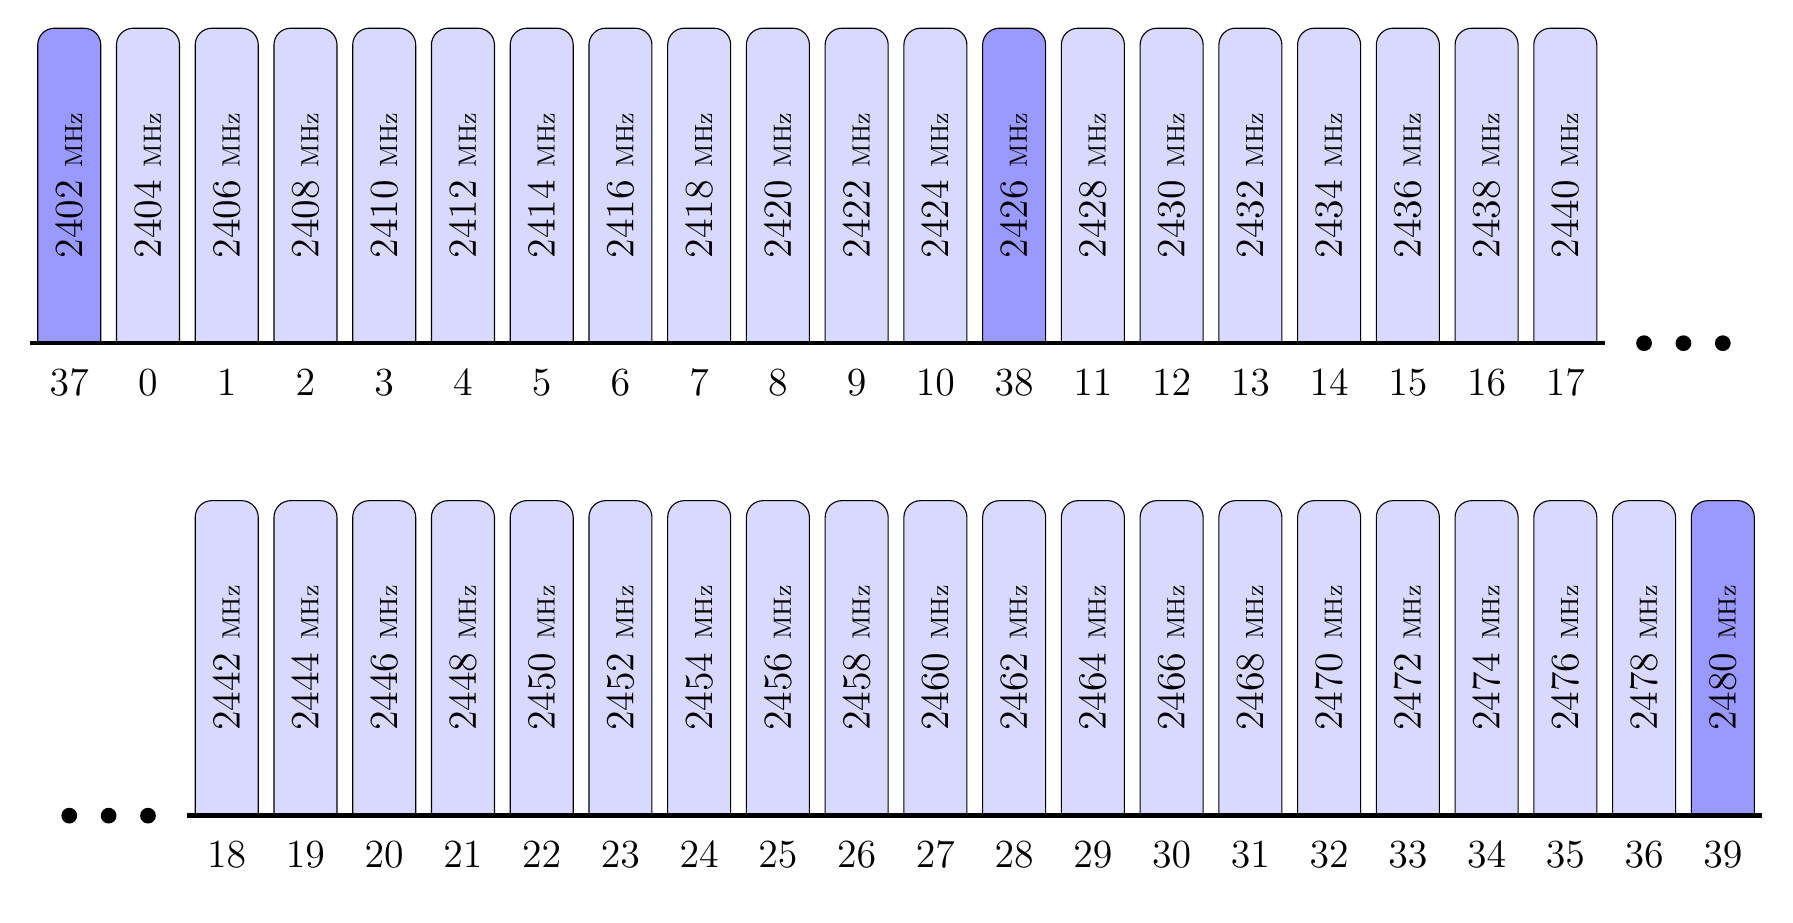
\begin{tikzpicture}
%\draw[gray] (0,0) grid (10,4);

\colorlet{regular_channel_fill}{blue!15}
\colorlet{advertise_channel_fill}{blue!40}

\foreach \x in {0,1,...,19}{
\fill[regular_channel_fill,rounded corners=0.6em](\x + 0.1, 0) -- ++(0,4) -- ++(0.8,0) -- ++(0,-4);
}
\foreach \x in {0,12}{
\fill[advertise_channel_fill,rounded corners=0.6em](\x + 0.1, 0) -- ++(0,4) -- ++(0.8,0) -- ++(0,-4);
}
\foreach \x in {0,1,...,19}{
\pgfmathsetmacro{\f}{int(2402 + 2 * \x)}
\draw[rounded corners=0.6em] (\x + 0.1,0) -- ++(0,4) -- ++(0.8,0) -- ++(0,-4);
\path (\x,0) rectangle ++(1,4) node[midway,rotate=90] {\Large$\f$ \small MHz};
}
\foreach \x/\ch in {0/37,1/0,2/1,3/2,4/3,5/4,6/5,7/6,8/7,9/8,10/9,11/10,12/38,13/11,14/12,15/13,16/14,17/15,18/16,19/17}{
\path (\x,-1) rectangle ++(1,1) node[midway] {\Large\ch};
}
\draw[ultra thick] (0,0) -- ++(20,0);
\foreach \x in {1,1.5,2}{
\fill (19.5 + \x, 0) circle [radius=0.1];
}

% Line two
\begin{scope}[xshift=-18cm, yshift=-6cm]
\foreach \x in {20,21,...,39}{
\fill[regular_channel_fill,rounded corners=0.6em](\x + 0.1, 0) -- ++(0,4) -- ++(0.8,0) -- ++(0,-4);
}
\fill[advertise_channel_fill,rounded corners=0.6em](39 + 0.1,0) -- ++(0,4) -- ++(0.8,0) -- ++(0,-4);
\foreach \x in {20,21,...,39}{
\pgfmathsetmacro{\f}{int(2402 + 2 * \x)}
\draw[rounded corners=0.6em] (\x + 0.1,0) -- ++(0,4) -- ++(0.8,0) -- ++(0,-4);
\path (\x,0) rectangle ++(1,4) node[midway,rotate=90] {\Large$\f$ \small MHz};
}
\foreach \x/\ch in {20/18,21/19,22/20,23/21,24/22,25/23,26/24,27/25,28/26,29/27,30/28,31/29,32/30,33/31,34/32,35/33,36/34,37/35,38/36,39/39}{
\path (\x,-1) rectangle ++(1,1) node[midway] {\Large\ch};
}
\draw[ultra thick] (20,0) -- ++(20,0);
\foreach \x in {1,1.5,2}{
\fill (17.5 + \x, 0) circle [radius=0.1];
}
\end{scope}


\end{tikzpicture}
}
\caption{The Bluetooth channel spectrum.}
\label{fig::bluetooth_spectrum}
\end{figure}\\
When it comes to network topology, the Bluetooth Low Energy standard is quite permissive in what it allows you to do. It is possible to simply broadcast to the surrounding world on some, or all, of the three advertising channels - this allows a device to send information to several other devices at the same time. However, it does have limitations; the information exchange is unidirectional only, so a broadcasting device cannot get anything in return.\\
\\
For fancier things, where you require more than just the capability to spew out advertising packets, there are \textit{connections}. In Bluetooth Low Energy, a connection is a periodic data exchange between \textit{one} central, and \textit{one} peripheral. It is not possible to send to two or more devices at the same time. Still, since Bluetooth 4.1, one physical device can don any combination of roles and connections it wants to. Thus, you can be a central and a peripheral at the same time. These \textit{instances} of centrals or peripherals are then free to connect to other centrals or peripherals.\\
\\
An important concept in Bluetooth Low Energy is the Generic Attribute Profile, or GATT for short. This is the workhorse behind virtually every BLE data transaction, and is what allows the standard to be so versatile. In essence, the GATT is simply a server-client type of service provided by Bluetooth, that allows for a standard way of organizing and accessing data.

\end{document}
